\documentclass[a4paper,parskip]{scrartcl}
\usepackage[usenames,dvipsnames,svgnames,table]{xcolor}
\usepackage[utf8]{inputenc}
\usepackage{amsmath}
\usepackage{enumerate}
\usepackage{textcomp}
\usepackage{fancyhdr}
\usepackage[a4paper]{geometry}
\usepackage{amsthm}
\usepackage{amsfonts}
\usepackage{graphicx}
%\usepackage{subfig}
\usepackage{subcaption}
%\usepackage{wrapfig}
\usepackage{float}

\bibliographystyle{apalike}


\author{Sven Jandura \& Edward Wang} 
\title{Dosimetry in Medical Physics}
\subtitle{Report of Results}

\geometry {
  top=0.75in,
  headsep=3ex,
  bottom=0.75in,
}

\fancypagestyle{plain}{
  \fancyhf{}
  \fancyhead[L]{Sven Jandura \& Edward Wang}
  %\fancyhead[C]{} %Center
  \fancyhead[R]{Page \thepage}
}

\renewcommand{\headrule}{\color{Black}\hrule height\headrulewidth\hfill}
\pagestyle{plain}

%\let\stdsection\section\renewcommand\section{\newpage\stdsection}

\newtheorem{mydef}{Definition}
\newtheorem{mythe}{Satz}


\begin{document}

\maketitle

\tableofcontents

\section{Introduction}

Brachytherapy is a common treatment for skin, breast, and prostate cancer, as well as for other tumors at various body parts. In the therapy, a radiation source is placed next to the tumor. The radiation then kills adjacent cancer cells \cite{Ref:1}.

To ensure the safety and effectiveness of the treatment, the spacial distribution of the radiation dose has to be known. This can either be obtained by a simulation using Monte-Carlo-Methods, or by measuring the dose distribution in a medium similar to human tissue. In this experiment, we employ both methods. We use a Strontion-90 radiation source, as commonly employed in Brachytherapy \cite{Ref:2}. We measured the dose distribution in water at different distances and angles to the source.  The simulation is done using the software \textit{FLUKA}. 

\section{Experimental Setup}

\subsection{Overview}

\begin{figure}
\centering
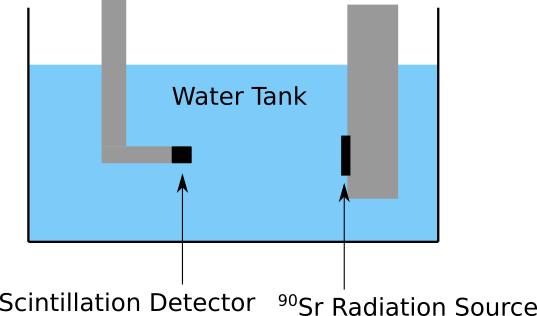
\includegraphics[width = 0.7\linewidth]{overviewCut.png}
\caption{Experimental Setup}
\label{Setup}
\end{figure}

The \textit{Absorbed Dose}, the quantity we measure in the experiment, describes how much energy is deposited by radiation per unit mass. It is measured in Gray (1~Gy~=~1~J/kg). Related quantities are the \textit{Equivalent Dose}, which is the absorbed dose weighted with a factor depending on the type of radiation, and the \textit{Effective Dose}, which is the equivalent dose weighted with a factor depending on the type of tissue irradiated, and thus describing the effect of the radiation on the human body.

In the experiment, we place the $~^{90}$Sr-Radiation source at a fixed point in a water tank. An Optidos\textsuperscript{TM} scintillation detector system is used to measure the radiation dose. It consists of a scintillation detector mounted on a three axis stepper motor, which allows translation in all three spacial directions. The detector is connected to a photomultiplier, which is in turn connected to a PC. The stepper motor are connected to the same PC. Both can be be controlled from a LabView program. The setup is shown in figure \ref{Setup}.

\subsection{Radiation Source}

We use a $~^{90}_{38}$Sr-Radiation source. $~^{90}_{38}$Sr decays to $~^{90}_{39}$Y via $\beta$-decay with a half-life of 28.79 $\pm$ 6~a, which the decays to $~^{90}_{40}$Zr again via $\beta$-decay with a half-life of 64 $\pm$ 21~h.  $~^{90}_{40}$Zr is a stable isotope \cite{Ref:2}. Our radiation source is disk-shaped with a diameter of 3mm.

\textit{Answer to Question 1:} The activity of the radiation source was measured at 9:47 a.m.
on 11th May of 2002 ($t_0$) to be $A(t_0) = 33.3 \pm 10\% \textrm{ MBq}$. (1 Bq means one radioactive decay per second). We assume, that at the time of this measurement, there where no $~^{90}$Y present. \footnote{This assumption is likely wrong, since it requires the time between the production or filtration of $~^{90}$Sr and the calibration of the source to be a lot shorter then 64 hours. If we instead assume, that $~^{90}$Y was at its equilibrium concentration during the calibration, the result of this and the following question have to be divided by two.} Then at the time of the experiment $t_{start}$ at 9 a.m. on November 12th 2018 ($t_{start}-t_0$=16.50~a) the activity due to $~^{90}$Sr  is:
$$A_{Sr}(t_{start}) = 2^{-(t_{start}-t_0)/t_{1/2}}A(t_0)$$
Since the half-life of $~^{90}$Y is a lot shorter than the half-life of $~^{90}$Sr, the concentration of $~^{90}$Y is always is a quasistationary equilibrium, that is, the number of $~^{90}$Y atoms that are created by the decay of $~^{90}$Sr per unit of time always equals the number of $~^{90}$Y atoms that decay to $~^{90}$Zr per unit of time. Hence, the total activity is twice the activity due to $~^{90}$Sr:
$$A(t_{start})= 2^{1-(t_{start}-t_0)/t_{1/2}}A(t_0) = 44 \pm 8 \textrm{MBq}$$
The activity is higher than at the time of calibration, since we now have $\beta$-decay due to $~^{90}$Sr and $~^{90}$Y.  

\textit{Answer to Question 2:} Since the activity satisfies 
$$A(t) = -\frac{\mathrm{d}N}{\mathrm{d}t} = -\frac{\mathrm{d}}{\mathrm{d}t}N(t_0)2^{-(t-t_{0})/t_{1/2}} = \frac{\log(2)}{t_{1/2}}N(t)$$
we have

$$N(t_0) = \frac{t_{1/2}A(t_0)}{\log(2)} = (1.0 \pm 0.3)10^{17}$$
So there where $10^{17}$ $~^{90}$Sr atoms in the source at calibration time.

\textit{Answer to Question 3:} Assume there are $N_0$ $~^{90}$Sr atoms at calibration time. Then at $t_{start}$, there are $N_{Sr}(t_{start}) = 2^{-(t_{start}-t_{0})/t_{1/2,Sr}}N_0 = (0.67 \pm 0.08)N_0$ $~^{90}$Sr atoms. There are $\frac{\log(2)}{t_{1/2,Sr}}N_{Sr}(t_{start})$ $~^{90}$Y atoms produced per unit time. Since the half-life of $~^{90}$Y is a lot smaller then the half-life time of $~^{90}$Sr, the concentration of $~^{90}$Y is in a quasistationary state, so there are also $\frac{\log(2)}{t_{1/2,Sr}}N_{Sr}(t_{start})$ $~^{90}$Y atoms decaying per unit time. Hence $A_{Y}(t_{start}) = \frac{\log(2)}{t_{1/2,Sr}}N_{Sr}(t_{start})$, so $N_Y(t_{start})=\frac{t_{1/2,Y}}{t_{1/2,Sr}}N_{Sr}(t_{start}) = (1.7 \pm 0.7)10^{-4}N_0$. The remaining atoms are $~^{90}$Zr, so $N_{Zr}(t_{start})=N_0-N_{Sr}(t_{start})=(0.33 \pm 0.8)N_0$.

\subsection{Scintillation Detector}
In the experiment, we use an organic scintillation detector. The dose deposited in the detector is comparable to the dose deposited in water or in human tissue. Thus, it is suitable to determine the dose distribution in water. The volume in which the radiation dose is measured is 0.8mm\textsuperscript{3}. The detector contains aromatic carbohydrate molecules. Ionizing radiation excites these molecules, which shortly after that ($10^{-9}-10^{-7}$s) to their ground state, emitting a photon in the process. These photons are guided through and optical waveguide to a photomultiplier, where the number of photons per unit time is measured. We used the Optidos\textsuperscript{TM} scintillation detector system, which provides the detector and the photomultiplier.    

The Optidos system was calibrated prior to the measurement in the following way: On October 13th 2015, a calibration was performed by the manufacturer. Right after this calibration, the dose deposited from the radiation source in a fixed position during a 60s interval was measured. The reading of the detector was $k_{p,0}=1171.0\frac{\mathrm{mGy}}{\mathrm{min}}$. Our experiment was conducted $3.08$ years after this calibration. We measured the radiation dose from the same source in the same position. If the sensitivity of the detector would have stayed the same since the calibration, we would expect a reading of $k_p = 2^{-3.08\mathrm{a}/t_{1/2,Sr}}k_{p,0}=1094.8\frac{\mathrm{mGy}}{\mathrm{min}}$. The uncertainty of $k_p$ is given by $\Delta k_p/k_p = \log 2 \cdot (3.08 \cdot \mathrm{a} \Delta t_{1/2})/(t_{1/2}) = 0.7\%$. So $k_p = (1095 \pm 0.7\%)\frac{\mathrm{mGy}}{\mathrm{min}}$ (Answer to \textit{Question 4}). We measure $k_m = 1087\frac{\mathrm{mGy}}{\mathrm{min}}$. The dose in water can then be calculated as 

$$D_W = 1.03\frac{k_p}{k_m}M$$

where $M$ is the reading on the detector. The prefactor 1.03 corrects for the type of radiation source, in our case a $~^{90}$Sr source.

Additionally to this calibration, the background radiation dose in the room was measured. However, it was below the measurement accuracy of the detector.

\section{Monte Carlo Simulations}
We use a Monte Carlo Simulation to calculate the dose distribution for our setup. In the simulation, a single particle leaving the radiation source is considered. It's energy and momentum are randomly sampled from the energy- and momentum distribution. The energy is distributed by a well known electron energy spectum for $\beta$-decay, the direction of the momentum is distributed uniformly. Then the path of the particle and possible interactions with the surrounding material are calculated. If those interactions produce secondary particles, their energy and momentum are sampled from the appropriate distribution. The procedure is stopped if the initial energy is completely deposited or all particles have left the simulation area. The dose deposited at each position is recorded. To obtain a dose distribution, this procedure is repeated for a large number of particles and the dose distribution in averaged over those runs.

In our experiment, we use the software \textit{FLUKA} for the simulation, and the GUI \textit{FLAIR} for FLUKA. In FLUKA, we simulated the dose distribution, taking into account the full geometry of the radiation source, including its shielding, and the geometry of the water tank, but not the scintillation detector. This is justified, since in the actual scintillator the deposited dose is approximately the same as it would be in water. This is not true for other parts of the detector, however, we minimize the influence of those parts by pointing the detector towards the source.

We simulated $10^9-1$ particles. 


\section{Experimental Results}

We approximated the $x$- and $y$- coordinate of our source by doing short scans with increasing resolution around the center. We get the approximations $x_0 = 26.9 \mathrm{mm}$ and $y_0 = 26.6 \mathrm{mm}$.

\subsection{Radial Direction}


We measured the dose distribution at constant $x=x_0$, $y=y_0$ for $z$ between 0 and 6mm. We expect that the intensity drops with a $\frac{1}{z^ 2}$ law. To verify this, we fitted the a curve of the form $\frac{A}{(z-z_0)^ 2}+I_0$ against the measured data. The result is shown in Figure \ref{radial_fits} (a). We approximate the uncertainty in $z$-direction to be $\pm 0.05 \mathrm{mm}$, since the stepper motor displays its position with a lowest digit of $0.1\mathrm{mm}$. The error for the intensity consists of a systematic and a random error. The systematic error comes mainly from the calibration and was estimated to $0.7\%$ in section 2.2. Since it affects all values by the same factor, we ignore it in the fit to $\frac{1}{z^2}$. The random uncertainty of the intensity is given by the Optidos-Software. For the first 12 value the uncertainty is given to be less the $0.5\%$. For value 13 and 14 it is given to be between $0.5\%$ and $1.0\%$. For the last 7 values, the uncertainty is given to be larger then $1.0\%$. We expect the relative random uncertainty to scale proportional to $N^ {-1/2}$, where $N$ is the number of particles the Optidos-System detects. $N$ should scale line $z^ {-2}$, so the random uncertainty should scale like $z^ {-1}$ Assuming that the uncertainty for value 14 is exactly $1\%$, we use this relation to estimate the error for the last 7 values. This leads to an uncertainty for $1.6\%$ for the last value.

We also fitted this dose distribution against the dose distribution we expect from the FLUKA-Simulation (Fig. \ref{radial_fits} (b)). This yields that the center of the source is at $-1.5 \mathrm{mm}$. Both fits give a good approximation of the data, but they deviate more that 3 times the estimated uncertainty from the measured data at multiple points. For both fits, the measured values are below the fit for $z \approx 2.5 \mathrm{mm}$ and above the fit for $z > 5 \mathrm{mm}$. We suspect that this is the case because we neglected the effects of the materials surrounding the scintillator. 

 \begin{figure}
 \centering
 \begin{subfigure}{0.7\linewidth}
 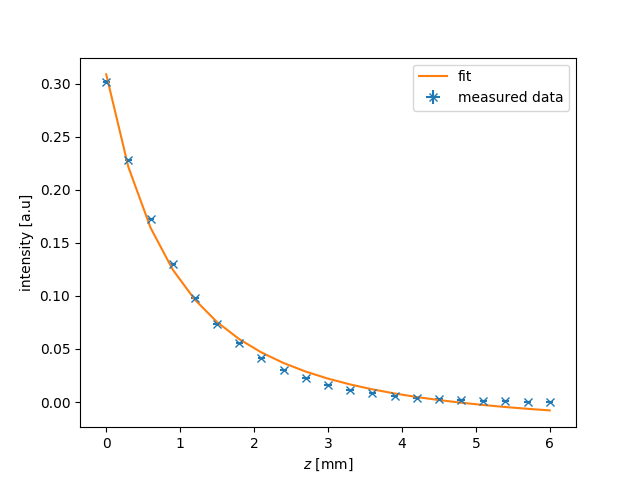
\includegraphics[width =\linewidth]{Fit_invers_quadratisch.png}
 \caption{}
 \end{subfigure}
  \begin{subfigure}{0.7\linewidth}
 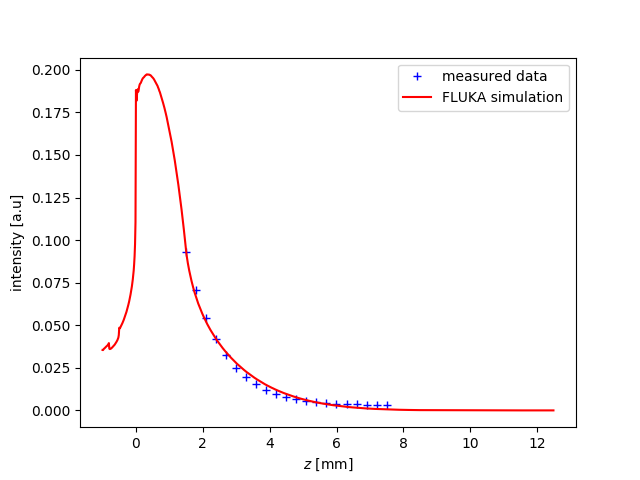
\includegraphics[width =\linewidth]{experiment_simulation_fit.png}
 \caption{}
 \end{subfigure}
 \caption{Fit of dose distribution with (a) a $r ^{-2}$ law and (b) the data from the FLUKA-Simulation}
 \label{radial_fits}
 \end{figure}

\subsection{Planes of constant $z$}

We measured the dose distribution in planes of constant $z$. The results for $z=0\mathrm{mm}$ and $z=3\mathrm{mm}$ are shown in Fig. \ref{2D Plots}. Both plots show the expected radial symmetry of the dose distribution.

\begin{figure}
\centering
\begin{subfigure}{0.49\linewidth}
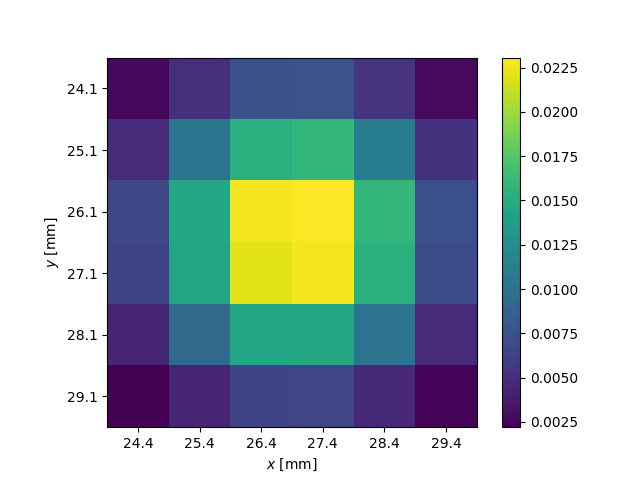
\includegraphics[width = \linewidth]{2D_Dose_Z0.png}
\end{subfigure}
\begin{subfigure}{0.49\linewidth}
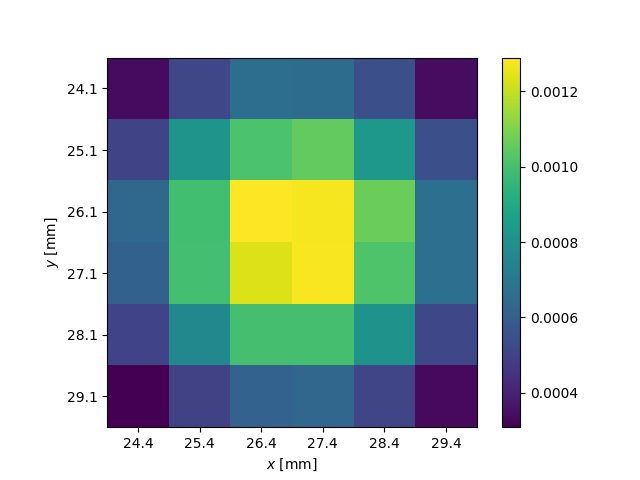
\includegraphics[width = \linewidth]{2D_Dose_Z3.png}
\end{subfigure}
\caption{Dose distribution at $z=0\mathrm{mm}$ (left) and $z=3\mathrm{mm}$ (right)}
\label{2D Plots}
\end{figure}

We also measured the dose distribution for fixed $z=0, x=x_0$ and varying $y$, as well as for fixed $z=0, y=y_0$ and varying $x$. We compared these results with the same results from the simulation. Based on the position of the source at $z=-1.5 \mathrm{mm}$ we used the plane with distance 1.5mm to the source when getting data from the simulation.  Both results are shown in Fig. \ref{plane-fits}. There are significant deviations between the measured data and the simulation. Part of the reason for that might again be, that the simulation neglected the materials surrounding the scintilator. However, according to \cite{Ref:2}, the deposited dose in the surrounding materials is between 80$\%$ and $110\%$ of the dose that would be deposited in water. Therefore, this effect cannot fully explain the deviations. We also note that the the measured data in $x$ and $y$ direction is almost identical, while in the simulation the distribution in $x$-direction is significantly broader then in $y$-direction.

In Fig. \ref{plane-fits} we aligned the data from the simulation with the measured data "by eye", This leads to a slight improvement of the values for $x_0$ and $y_0$: We get $x_0=27.1 \mathrm{mm}$ and $y_0 = 16.8 \mathrm{mm}$. Thus, in both coordinates our initial approximations where off by 2mm.

 \begin{figure}
 \centering
 \begin{subfigure}{0.7\linewidth}
 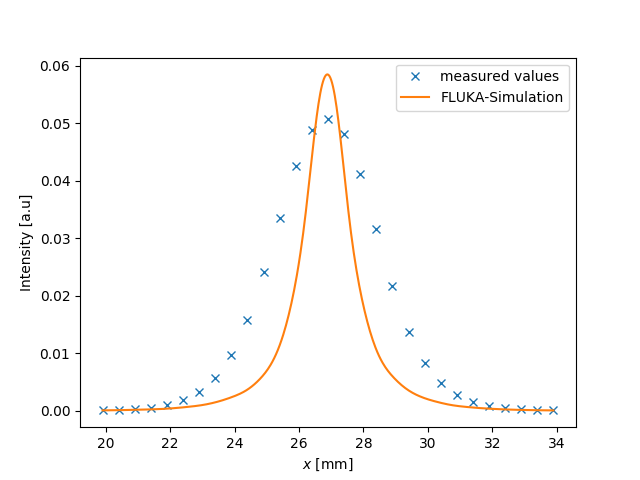
\includegraphics[width =\linewidth]{xScanZ0.png}
 \caption{}
 \end{subfigure}
  \begin{subfigure}{0.7 \linewidth}
 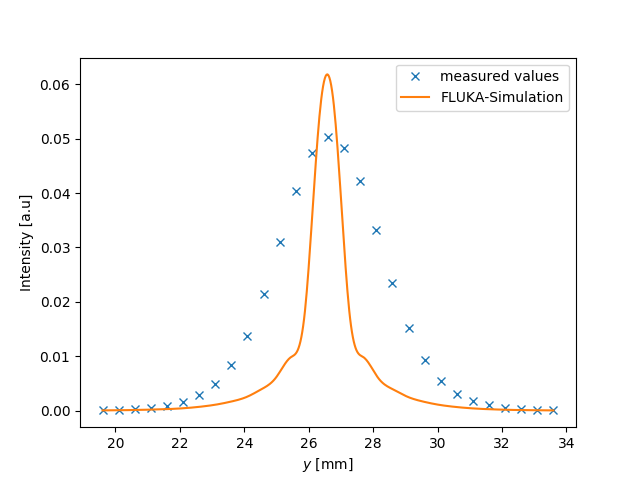
\includegraphics[width =\linewidth]{yScanZ0.png}
 \caption{}
 \end{subfigure}
 \caption{Comparison of measured values and simulation results in (a) $x$- direction and (b) $y$ -direction}
 \label{plane-fits}
 \end{figure}

\section{Summary}

In this experiment, we measured the three dimensional dose distribution of a $~^ {90}$Sr-Source in a water tank to simulate the dose deposition in medical applications, like Brachytherapy. We also simulated the dose distribution using the software FLUKA. The results of the simulation and the measurements agree with slight deviations in the radial direction. For planes of constant $z$, the results of the simulation and the measurement differ significantly. These deviations might be explained partially by the negligence of the materials surrounding the scinitallator in the simulation. 

\newpage

\bibliography{reference}

\end{document}

